%% Author_tex.tex
%% V1.0
%% 2012/13/12
%% developed by Techset
%%
%% This file describes the coding for rsproca.cls

\documentclass[]{rsos}%%%%where rsos is the template name

\usepackage{lineno}
\linenumbers

\usepackage[T1]{fontenc}
\usepackage[utf8]{inputenc}


% tightlist command for lists without linebreak
\providecommand{\tightlist}{%
  \setlength{\itemsep}{0pt}\setlength{\parskip}{0pt}}

% From pandoc table feature
\usepackage{longtable,booktabs,array}
\usepackage{calc} % for calculating minipage widths
% Correct order of tables after \paragraph or \subparagraph
\usepackage{etoolbox}
\makeatletter
\patchcmd\longtable{\par}{\if@noskipsec\mbox{}\fi\par}{}{}
\makeatother
% Allow footnotes in longtable head/foot
\IfFileExists{footnotehyper.sty}{\usepackage{footnotehyper}}{\usepackage{footnote}}
\makesavenoteenv{longtable}


\usepackage{float}
\usepackage{booktabs}
\newcommand{\beginsupplement}{ \setcounter{table}{0}     \renewcommand{\thetable}{S\arabic{table}}\setcounter{figure}{0} \renewcommand{\thefigure}{S\arabic{figure}}}

%%%% *** Do not adjust lengths that control margins, column widths, etc. ***

%%%%%%%%%%% Defining Enunciations  %%%%%%%%%%%
\newtheorem{theorem}{\bf Theorem}[section]
\newtheorem{condition}{\bf Condition}[section]
\newtheorem{corollary}{\bf Corollary}[section]
%%%%%%%%%%%%%%%%%%%%%%%%%%%%%%%%%%%%%%%%%%%%%%%

\begin{document}


%%%% Article title to be placed here
\title{Combination of field and experimental data together with computational models reveal cognitive mechanisms behind cleaner fish behaviour}

\author{
Andrés E. Quiñones$^{1}$,
Zegni Triki$^{2}$,
Redouan Bshary$^{1}$}

\address{
  $^{1}$Institute of Biology, University of Neuchâtel, Neuchâtel, Switzerland\\
  $^{2}$Department of Zoology, Stockholm University, Stockholm, Sweden}
%%%% Subject entries to be placed here %%%%
\subject{
Behavioural ecology,
Cognitive ecology,
Animal behaviour}

%%%% Keyword entries to be placed here %%%%
\keywords{
learning,
cleaners,
behaviour,
bayesian statisitics,
mutualism}

%%%% Insert corresponding author and its email address}
\corres{
  AE. Quiñones\\
  e-mail: \href{mailto:andreseqp@gmail.com}{\nolinkurl{andreseqp@gmail.com}}
}

%%%% Abstract text to be placed here %%%%%%%%%%%%
\begin{abstract}
While it is generally straightforward to quantify individual performance in cognitive experiments, identifying the underlying cognitive processes remains a major challenge. Often, different mechanistic underpinnings yield similar performances, and Lloyd Morgan's cannon warrants acceptance of the simpler explanation. Alternatively, when the different mechanisms interact with environmental conditions, variation in performance across environments might allow to statistically infer the mechanism responsible. However, to do this it is necessary to have quantitative predictions for the different candidate mechanisms. Here, we use a set of computational models to get quantitative predictions from alternative learning mechanisms, and using Bayesian statistics fit the model parameters to performance data. We used experimental data on performance in an ephemeral reward task by wild-caught cleaner fish \emph{Labroides dimidiatus}, as well as cleaner and client fish densities from the locations of capture. The task can in principle be solved by estimating future consequences of an action, or by perceiving the removal of the ephemeral reward as psychological punishment (negative reinforcement). We found that a model where cleaners only estimate the future consequences of their actions explains best which cleaner relative abundances cause the fish to develop a preference for an ephemeral food source. This model also yields performances that can be considered the result of locally optimal decision-rules, in contrast to the negative reinforcement model. We argue that the combination of computational models with data is a powerful tool to infer the mechanistic underpinning behind cognitive performance.
\end{abstract}
%%%%%%%%%%%%%%%%%%%%%%%%%%%

\providecommand{\EndFirstPage}{%
}

\maketitle

\hypertarget{introduction}{%
\subsection{Introduction}\label{introduction}}

Disentangling the mechanistic underpinnings of behaviour
is typically done under controlled conditions in a laboratory setting. However,
controlled laboratory conditions often mask the inter and intra-specific
variation that arises in the interaction between mechanisms and
environmental variation. From a evolutionary perspective, mechanisms
are likely selected because of how they allow individuals to respond to
environmental variation. For example, biological market theory predicts that
the exchange rate of goods and/or services traded between cooperative
partners adjusts to the law of supply and demand, when individuals have
some degree of partner choice \citep{noe_Biological_1995a}.
Supply and demand conditions, which typically
depend on the abundance of the species involved, certainly vary in time
and space. Therefore, natural selection should
favour the ability to flexibly adjust decisions and behavioural output to
current market conditions. Indeed, such adjustments have been repeatedly
documented \citep{axen_Signalling_1996}. In animals, an obvious general candidate
mechanism for the strategic adjustment is the cognitive machinery. However,
it is not clear which cognitive mechanisms allow individuals to adjust their
behaviour to the varying market conditions. As adjustments to changes in
market conditions have been documented in a great variety of species with
highly variable brain anatomies, the question arises to what extent mechanisms
beyond basic associative learning may be involved.

One example of strategic adjustment in a biological market is the marine
cleaning mutualism involving the cleaner fish \emph{Labroides dimidiatus} and
`client' fish. Client fish seek cleaner fish services at their territory
(so-called ``cleaning station'') and offer themselves as food patches
to get their ectoparasites removed, which provides cleaners
with food and clients with improved health \citep{waldie_LongTerm_2011, ros_Does_2011, triki_Effects_2016, demaire_Reduced_2020}.
Given the capacity of some client fish to swim larger distances and
access multiple cleaning stations while others access the only cleaning
station at their territory, it is crucial to categorize clients as
either ``visitors'' or ``residents'', respectively. During cleaning interactions,
a cleaner fish often face a choice between a visitor and a resident client
seeking its cleaning services simultaneously. Visitors have the option
to switch to another cleaner fish if being made to wait, while residents
must wait for inspection. Indeed,
visitors have been observed to use their partner choice option in that
way \citep{bshary_Choosy_2002}, which may explain why cleaners give
visitors service priority in a field study in the Red Sea
\citep{bshary_Cleaner_2001a}.

When researchers aimed at testing wild-caught cleaner fish, as
well as individuals from other species, abilities
to prioritize visitor over resident clients in a lab-based paradigm,
they used Plexiglas plates of different colours and shapes offering same
amount of food as surrogates for visitor and resident clients.
One plate is made to behave like a resident, i.e.~it remains until
the cleaner had eaten off it. The other plate was made to behave
like a visitor, i.e.~it is removed if not inspected first.
Cleaners learned to prefer the visitor plate and
hence obtained the double amount of food \citep{bshary_Asymmetric_2002}.
Furthermore, adult cleaner fish outperformed various primates as well as rats and
pigeons in this original version of the biological market task
\citep{salwiczek_Adult_2012, zentall_Early_2017}; yet the African grey
parrots solve this task as well \citep{pepperberg_Can_2014}. Given that primates
are known to readily distinguish
between one and two reward units if presented in more conventional ways
\(\color{red}{\text{ref}}\), this raises the question:
what makes the task difficult for most non-cleaners?

Recent research on the cognitive tool kit needed to solve the ephemeral
reward task has used a broad approach as proposed by Shettleworth
\citep{shettleworth_Cognition_2009}, who defined cognition as including
all ways in which animals acquire information
through the senses, process, retain and decide to act on it.
Indeed, perception of relevant cues is of major importance
for individual performance. For example, some animals find relevant
information in the plates
\citep{wismer_Cuebased_2019}) while others find it in the food
\citep{pretot_Comparative_2021, pretot_Comparing_2016}. However, identifying
cues as salient is not the only challenge of the ephemeral reward task,
as revealed by proximate learning models. Such models allow varying the
cognitive tool kit and to evaluate which minimal kit is necessary to solve
the task at hand (e.g. \citep{dubois_Model_2021}). Applied to the ephemeral
reward task, learning models showed that basic reinforcement learning does
not suffice to solve the ephemeral reward task \citep{prat_Modelling_2022, quinones_Reinforcement_2019}.
This is particularly so when models assume the more complex natural
situation in which cleaner fish not only face resident-visitor pairs but also
visitor-visitor and resident-resident pairs, as well a resident alone or
a visitor alone. To be able to give visitors priority over residents,
cleaners need to be able to assess a client's value separately for the
three possible scenarios (alone, paired with a fish with the
same strategic option, paired with a fish with the alternative strategic option)
\citep{quinones_Reinforcement_2019}. The ability to distinguish and value differently
one stimulus alone from compound versions of it has been termed
configurational learning, or chunking,
or segmentation (see references in \citep{prat_Modelling_2022}).

To solve the ephemeral reward task, cleaners need to account for
the future consequences of current decisions. In the model by
Quiñones \emph{et al.} \citep{quinones_Reinforcement_2019}, this could be achieved in
two non-mutually exclusive ways: through low temporal discounting of
future effects, also termed `chaining' \citep{enquist_Power_2016}; and/or
through perceiving a visitor client leaving as psychological punishment
(i.e.~as a negative reinforcer). Low temporal discounting is when
individuals include in their valuation of an action the reward effects
that this will have in the future. This is done by combining in a single
valuation the reward obtained in the current time with all the reward that
comes after, discounting for how far in the future the future reward
is accrued. `Chaining' the reward of these different time steps allows
individuals to take actions that increase the long-term reward at the sacrifice
of short term considerations \citep{enquist_Power_2016}. Even though, `chaining'
can be readily implemented computationally in learning models
\citep{enquist_Power_2016, sutton_Reinforcement_2018}, cognitively it seems to be
a complex adaptation \citep{suddendorf_Evolution_2007}. On the other hand,
using client behaviour as a negative reinforcer is in principle
easier to implement. Negative reinforcement is part of the ubiquitous
learning mechanism termed operant conditioning \citep{thorndike_Animal_1898, skinner_Behavior_1938}. Thus, standard logic of
Lloyd Morgan's cannon demands that operant conditioning as the simpler
explanation is to be accepted by default. Ideally, the two mechanisms should
be evaluated in light of how well they explain the available data.

Over the last decade, our team tested over a hundred of wild-caught
cleaner fish in the exact same paradigm of of the ephemeral reward
task \citep{salwiczek_Adult_2012, wismer_Variation_2014, triki_Decrease_2018, triki_Biological_2019, triki_Brain_2020}. These fish often come from
different reef locations around the study field site at Lizard Island,
Great Barrier Reef in Australia. Further investigation of the local
eco-sociological conditions revealed that cleaner and client
fish population densities have a substantial impact on cleaner fish
performance in the task. Cleaner fish from reef sites with relatively
low densities were more likely to fail solving the task \citep{triki_Biological_2019, triki_Decrease_2018, wismer_Variation_2014}. The explanation for this pattern
is twofold. First, low cleaner fish population densities imply
low supply and high demand for cleaning services.
Under such conditions, there are fewer occasions under
which failing to give priority to a visitor translates to an empty
cleaning station. Second and also related to the state of the cleaning market,
visitor clients at low cleaner fish population densities
are less likely to exert their partner choice options
and are hence more likely to wait for inspection if not given cleaning
priority \citep{triki_Brain_2020}. In the absence of partner choice
cleaners should not give priority to visitors any more.

The interplay between the underling cognitive machinery and
local ecological conditions apparently generate the documented variable
performance among individuals of the same species.
Our approach of fitting the computational model to the empirical data on
fish densities and cleaner fish censuses and cleaner fish performance
in the ephemeral reward task aimed at: (i), determining which
mechanism cleaner fish use to incorporate future consequences of current
decisions by testing whether operant conditioning, chaining, or a combination
of both best explains their performance; (ii) determining whether the
two mechanisms differed with respect to the ecological conditions
that are likely to cause high versus low performance in the
ephemeral reward task. Additionally, we assessed which mechanism
yields optimal performance patterns. Relying on the logic of
biological market theory, we predicted
that appropriate performance is to show low preference for visitors under low
local cleaner-to-client ratio. In this case, as visitor leaving rates
should be low as well and any leaving visitor will be readily
replaced by another client in the queue. In contrast,
cleaners should show high performance in the ephemeral reward task
if the local cleaner-to-client ratio favours clients.

\hypertarget{methods}{%
\subsection{Methods}\label{methods}}

\hypertarget{overview}{%
\subsubsection{Overview}\label{overview}}

To test the relative validity of chaining versus negative reinforcement as
mechanisms to account for future consequences of current choices,
we combined empirical data from Triki \emph{et. al}
\citep{triki_Biological_2019, triki_Brain_2020}. with the computational
model analysed in Quiñones \emph{et al.}\citep{quinones_Reinforcement_2019}. In order to
compare the explanatory power of the different hypothesis, we estimate the
parameter values of three versions of the model that best fit the data.
Particularly, we fit the parameter that determines how important
future rewards are (\(\gamma\)), the magnitude of the negative reward
(\(\eta\)) and a scaling constant that translates absolute to relative
abundances (see following sections for details). We obtained model
predictions using a set of stochastic individual-based
simulations. Thus, each parameter combination of the model yields not one
prediction for the data set, but a distribution of them. Thus, for the
fitting procedure, we use one of the most common algorithms in bayesian inference,
the Markov Chain Monte Carlo (MCMC). MCMC is a stochastic algorithm that allows
to sample from the posterior distribution of model parameter values. The posterior
distribution represents the most likely parameter values given the data.
Due to the stochastic nature of MCMC, which repeatedly samples parameter values
and evaluates their likelihood, the distribution of likelihoods from the
stochastic model is also explored. This makes MCMC and bayesian inference
particularly suitable for the computational models we evaluate. Bellow,
we explain first the computational model and the data collection, and later
how the MCMC was used to estimate parameter values.

\hypertarget{the-model}{%
\subsubsection{The model}\label{the-model}}

The model consist of a set individual-based simulations where
individuals face a series of choices between two options. Individuals in
the model represent cleaners, and the options they face simulate the
natural conditions of a cleaning market. Cleaners experience a series
of discrete time points in which they face different `states', which
are defined by the number and type of clients inviting for service.
There are six possible states: zero clients, one resident, one visitor,
two residents, two visitors, and a mix of one resident and one visitor.
The probability of each state is largely determined by the relative
abundance of cleaners, residents and visitors, but to some degree by a
cleaner's choices when it faces the resident-visitor combination.
This is because residents are those clients that stay in the
cleaning queue when they are not given priority and hence would
still be available in the next time point; while visitors leave
the queue (with a certain probability) after they are not given
priority. Individuals obtain a fixed reward from cleaning a client
regardless of the type. Every time individuals face and make a choice
they update the probability of making that same choice. The update is
based on the difference between the expectation of reward and the actual
reward the individual obtains (prediction error)
\citep{sutton_Reinforcement_2018, rescorla_Theory_1972}; and it is carried
in the direction that would lead to more reward being obtained, given
the new information. In the long run, the probability of choosing a visitor
over a resident converges in the model. To which probability the model
will converge depends on the relative abundance of cleaners, visitors
and resident; as well as on the probability of visitors leaving the station
when unattended. Further details of the model implementation can be
found in the paper \citep{quinones_Reinforcement_2019}.

The model shows that only agents that calculate rewards separately for
the different states (termed `fully aware agents') can potentially
prioritise visitors of residents in nature, and hence also solve the
ephemeral reward task. This is because pooling rewards for the two
clients from all states by `partially aware agents'
(that only recognize the two clients as different) cancels out
all differences (see \citep{quinones_Reinforcement_2019}). However,
such \emph{chunking} by fully aware agents is not enough to develop a
preference for visitors. In addition, agents need to find a mean
to incorporate future consequences of current choices. In the model,
this could be achieved with either of two parameters that could
also work together. First, \(\gamma\) measures how
much individuals include future rewards in their decision updates. If
\(\gamma=0\), individuals only use the immediate reward obtained from a
cleaning interaction. As \(\gamma\) increases individuals include more the
reward obtained from the subsequent choices. That amounts to calculating
and using for decision making the future expected rewards of an action.
Second, \(\eta\) measures how much individuals include in their reward the
fleeing behaviour of visitor clients as a negative component. Both of
these parameters allow individuals to use in their estimates the future
effects of their choices.

A further model analysis contrast the effect of these two
parameters against variation in the relative abundance of cleaners
and the two client types. Assuming certainty that visitors leave, the
two parameters yield different
predictions when relative client abundance is very high. Under such
conditions, the analysis shows that under very high client (relative)
abundance the presence of future rewards (\(\gamma>0\)) no longer favours
the preference for the ephemeral clients, while the preference persists
when the negative reward mediated by client behaviour (\(\eta>0\)) is
included. Thus, the analysis suggests that future reward as an
explanation for cleaner ability to prefer visitors is supported.
At first sight, empirical data seem to support future rewards as
the mechanism used by cleaners, as the statistical analysis by
Triki \emph{et al.} \citep{triki_Biological_2019} data revealed that low
cleaner-to-client ratios predict low preference for visitors and hence
low performance in the ephemeral reward task. However, low cleaner-to-client
ratios may also lead to low probabilities of visitors leaving, which would
cause low preferences for visitors independently of the underlying
mechanism \citep{quinones_Reinforcement_2019}. Furthermore, a combination
of future and negative rewards, could still be yield a better explanation
for the data than any single factor.

\hypertarget{empirical-data}{%
\subsubsection{Empirical data}\label{empirical-data}}

The empirical data were collected between 2010 and 2018 always during
the austral winter months June to August at Lizard Island
(\(14.6682° S, 145.4604° E\)), Great Barrier Reef, Australia.
They consist of three sets: fish densities from a total of five study
reef sites (Corner Beach-CB, Horseshoe-HS,
Mermaid Cove-MC, Northern Horseshoe-NHS, and The Crest-TC),
natural observations of cleaners to quantify the probability
of visitors leaving if initially ignored in favour of another client, and the
performance of individuals caught from these sites in the ephemeral reward test.
In total, we have twelve site/year data sets for fish densities and
corresponding performance in the test. Thus, some sites were sampled more
than once. Due to major environmental perturbations during the study period
(\(\color{red}{\text{refs}}\)), fish densities changed significantly even
within sites \citep{triki_Decrease_2018, triki_Fluctuations_2019}. To estimate
the population density of cleaner fish and their clients at a given site in
a given year, Triki \emph{et al.} \citep{triki_Biological_2019} used a series of ten
transects of \(30m\) each. Observers swam along the transect lines placed on
the reef and first counted the visible large-bodied adult fish
(species with total length TL \textgreater{} \(10cm\)) on a width of \(5m\), and then on the
return individuals of small-bodied fish species (TL \textless{} \(10 cm\)) on a width
of \(1 m\). We included cleaner fish in the \(5 m\) transect. Based on the
classification by Bshary \citep{bshary_Cleaner_2001a} and Wismer \emph{et al.}
\citep{wismer_Variation_2014}, all visitor client species (\(n = 124\)) were
large-bodied. Resident clients comprised all small-bodied species
(\(n = 30\)) but also some large-bodied ones (\(n = 15\)). Overall,
large-bodied species are highly correlated with being a visitor,
and small-bodied species are a good correlate of residents. Based on the
transect data, Triki \emph{et al.} \citep{triki_Biological_2019, triki_Brain_2020}
estimated cleaner fish, small-bodied client, large-bodied client and total
client fish densities per \(100 m^2\). LASSO analyses revealed that cleaner and
large-bodied client densities were highly correlated, and only the former
was hence kept in the analyses as representative of both \citep{triki_Biological_2019}.
Cleaner densities, in interaction with visitor client leaving probability,
explained best individual performance in the ephemeral reward task
\citep{triki_Biological_2019}, while cleaner-to-client ratio was not a significant
factor. This creates a certain mismatch with the model by Quiñones \emph{et al.}
\citep{quinones_Reinforcement_2019}, which focused on abundance of cleaners relative
to overall client abundance in order to capture the characteristics
of the market. Importantly, relative abundances of clients define not only
the probability of interactions with residents and visitors, but also affect
how often the cleaning station is empty (e.g.~there are no clients to be cleaned).
The higher the relative abundance of cleaners is, the higher is the probability
of cleaning stations being empty at a given time point. How often the
cleaning stations are empty in turns influences the value that cleaners can
expect from their choices. The emptier the cleaning stations are, the more
beneficial it is to prioritize a client that will not stay. On the other hand,
situations where cleaners have to choose will be rare if cleaner relative
abundance is high, which reduces the total value of prioritizing visitors
over residents and makes it more difficult to learn a preference for visitors.
Given the model structure, we used the empirical data to calculate relative
abundances of cleaners, residents and visitors for the current analyses.
To incorporate the empirical finding that absolute densities matter, we
introduced a new scaling constant (see section on model fitting).

To collect data on the visitor clients' probability of leaving if not serviced
immediately, eight cleaners per site/year were each filmed for \(30 min\).
From the videos, all events in which a visitor client was made to wait in
favour of another (visitor or resident) client were identified, and noted
whether or not the visitor left \citep{triki_Biological_2019, triki_Brain_2020}.
A total of 120 cleaners (10 individuals per 12 site/year) were tested in the
ephemeral reward task \citep{triki_Biological_2019, triki_Brain_2020}. Authors
housed all captured cleaners individually in glass aquaria
( \(62cm \times 27cm \times 37 cm\) ) and provided them
with PVC pipes (\(10 cm \times 1 cm\)) as shelters.
The task consisted of exposing the cleaner fish to substitute
models of client fish in the form of two \emph{Plexiglas} plates offering the
same amount of food (one item of mashed prawn). The two plates differed
in colour and pattern (horizontal green stripes or vertical pink stripes)
but had equal size (\(10 cm \times 7 cm\)). Importantly, the two plates played
different roles as either a visitor (ephemeral food source) or
resident (permanent food source). That is, if a cleaner inspected the
resident plate first, the experimenter withdrew the visitor plate out of
the aquarium as a consequence. Choosing first the visitor plate,
however, granted access to both plates. The equal size of the plates
forced cleaner fish to learn to give service priority to the visitor plate
based solely on the behaviour-cue of the plates rather than size-cue
\citep{wismer_Cuebased_2019}. Triki \emph{et al.} \citep{triki_Biological_2019, triki_Brain_2020}
tested the fish for a maximum of 200 trials with 20 trials a day, 10 trials
in the morning and 10 trials in the afternoon. They randomized and
counterbalanced the plates' spatial location (i.e.~left or right)
between trials. Similarly, they counterbalanced the plates' decoration
(colour and pattern) and the plates' role (visitor or resident) between the
tested fish. The data was originally collected to assess which variables are
good predictors of the capacity to solve the ephemeral food task. Thus, previous
analysis use specific statistical criteria to classify individual cleaners'
performance as successful or failure \citep{triki_Biological_2019}. Because the model
predicts the preference of cleaners given the set of environmental variable,
we instead use the raw data of individuals cleaners' decisions.
We use 20 choices from each cleaner as the preference they develop
for the visitor plate. Which these 20 choices were vary for each cleaner depending
on the performance that was originally assessed. For cleaners that did not
succeed, the 20 choices correspond to the last two sessions. Cleaners that
succeeded in solving the task were tested on a reversal task. That is, the
pattern in plates was switched to the opposite role they played in the
initial test. For those cleaners, we used the last session before they succeeded
in the initial, and the last session of the reversal, completing the 20 choices.
We did not distinguish between individuals that reached the criterion early
or late during the 200 trials.

\hypertarget{statistical-analysis}{%
\subsubsection{Statistical analysis}\label{statistical-analysis}}

The aim of the analysis is to fit the key model parameters that allow
individuals to incorporate future consequences of current actions,
\(\gamma\) and \(\eta\), to the data from Triki \emph{et al.}
\citep{triki_Biological_2019, triki_Brain_2020} to find out whether each or
a combination of these effects is a better explanation for the pattern
seen in the data. In particular, we are interested in the relation between the
ecological variables: cleaners, visitor clients, resident clients abundances and
visitor clients leaving probability; and cleaners' preference for visitor clients
over residents. Thus, the four ecological variables are given as input to
the models. The preference for visitors gotten from the simulations of the model
is used as the prediction for the response variable, while the number of visitors
chosen out of the 20 choices of each cleaner as the observed response variable.
We kept all other parameter values used for the model simulations constant,
see Table \ref{tab:param}.

In order to capture with the model the relationship between the characteristics
of the market (environment) and the cleaner's preference we need to translate
the absolute abundances of the data to to a measure of relative abundances
that captures client visitation patterns. This is because in the model, relative
abundances of clients define not only the probability of residents and visitors,
but also how often the cleaning station is empty (e.g.~there are no
clients to be cleaned). The frequency with which clients visit the station
is another variable, which will likely vary among different client species
depending on parasite abundances and loads. We do not have field estimates
for species specific parasite loads, especially not as a function of site.
In order to control for these aspects, we computed a measure of relative
cleaner abundance for each site relative to absolute abundances and multiplied
by a scaling constant that changes the range of the variable. This scaling
constant is hence meant to capture variation in the market conditions driven
partly by cleaner abundance. We fit the value of the scaling constant as
part of the statistical inference. As for the client abundances for
residents and visitors we computed a relative measure with respect to the
total client abundance, and weighted that by the rescaled relative absence
of cleaners (\(1-\text{relative cleaner abundance}\)). Thus, all three measures
of relative abundance sum up to 1, and can be used in the model as a proxy
for the probability of having different options in the cleaning station.
Note that the scaling constant was introduced to control for variation that
is not captured by the model; its parameter distribution does not offer
biological insights.

Once we calculate the relative abundances, we can obtain predictions from
the model for each one of the locations and run the Markov Chain. We start the
chain with random values for the parameters of interest, then run the
computational model once for every location using as input the ecological
explanatory variables. The model outputs the probability of choosing the visitor
for each location \(p_i\), where \(i\) is the index for the 12 locations. Assuming a
binomial distribution, the probability that each of the cleaners' 20 choices was
generated by the model is given by \(\binom{n}{k_ij}p^{k_{ij}}_i (1-p_i)^{n-k_{ij}}\);
where \(k_{ij}\) is the number of times that cleaner \(j\) in location \(i\) chose the
visitor over the resident; and \(n=20\) (due to our choice of using 20
choices per cleaner). By taking the natural logarithm and summing over all
the cleaners and locations we obtain the log-likelihood of the data
given the model and parameters. We then propose a new set of parameters drawn
from a uniform distribution centred around the old parameter set. The amplitude
of the uniform distribution used for each parameter can be found in Table
\ref{tab:param}. Subsequently, we ran the model and calculated the likelihood
with the new parameter set. We then use the ratio of the two likelihoods to
choose which parameter set to keep. New parameter sets with a higher likelihood
than the old set replace old ones, and those with a lower likelihood are replace
current ones with a probability equals to the log-likelihood ratio.
Given that we only use the likelihoods in the decision, we are using a
uninformative prior. Once we decide whether the new parameter set replaces
the old one, we ran the model again to sample to the likelihood
distribution of the parameter set. We then start
the cycle again by proposing a new set of parameters, and repeat the process for
\(1e^5\) steps. We ran 5 independent chains, discarded the first
\(100\) samples of each chain as burn in, and after that we keep 1 in every
100 samples to avoid autocorrelation. The collection of parameters sets kept in
all chains approximates the posterior distribution. The model as well as the
fitting algorithm were coded in \emph{c++}, the diagnostics and visualization were
coded in R \citep{rcoreteam_Language_2021} of the all code can be found at
\(\color{red}{\text{include citation}}\)

In order to compare the fit that the three alternative models give we use the
distribution of pseudo \(R^2\) proposed by Mcfadden \citep{mcfadden_Conditional_1974}.
Mcfadden's pseudo \(R^2\) is a standard measure of fit for logistic regression.
In that context, \(pseudo-R^2\) uses the log-likelihood of the data given
the model, relative to the log-likelihood of the data given a
model without covariates, as a measure of fit. Given that our
model is not a logistic regression, we measure the \(pseudo-R^2\) in
relation to the log-likelihood of a model
with parameters \(\gamma\) and \(\eta\) set to zero. This in practice
amounts to a model that has neutral preference between the two options.
Pseudo \(R^2\) was calculated for all the samples of the posterior gotten from
the MCMC. Thus, we use these distributions of pseudo \(R^2\)'s as a measure of
fit.

\hypertarget{results}{%
\subsection{Results}\label{results}}

\begin{figure}

{\centering 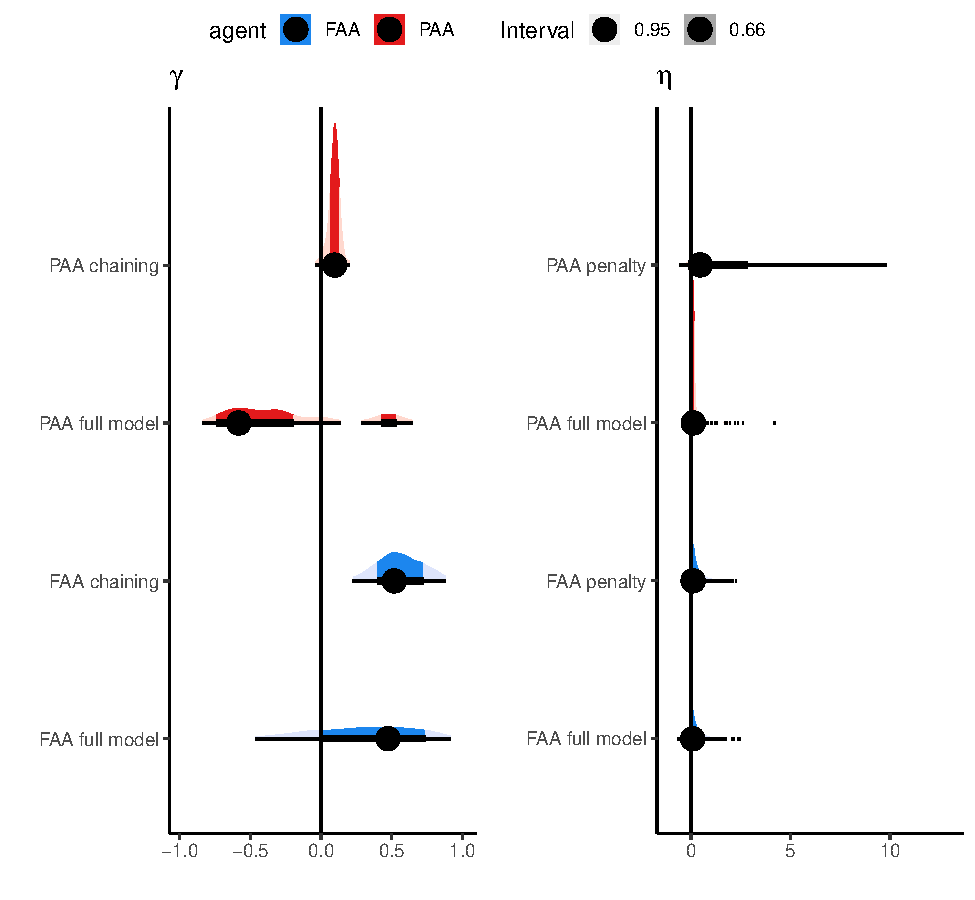
\includegraphics[width=1\linewidth]{manuscript_1.0_files/figure-latex/post-1} 

}

\caption{Posterior distributions for parameter values $\gamma$, $\eta$ and the scaling constant. We show the kernel density estimates, below the mode (black point) and the 65\% (light blue) and 95\% (grey)  highest posterior density interval for the three paramteres. On the left (panels a, c and c) posterior distributions for a model with all three parameters; while on the right (b and d) a model without negative reward. Panel f shows a measure of fit for both models, namely the distribution of pseudo-$R^2$ obtained from sampling the posterior distribution of parameter values.}\label{fig:post}
\end{figure}

Figure \ref{fig:post} panels a,c and e show the posterior distributions
of the parameter values of the full model, which includes both future
and negative reward. Posterior distributions show the probability
density (y axis) of the estimated parameter values (x axis). Notably,
the bulk of the posterior distribution for the parameter tuning negative
reward (\(\eta\) panel e) is around zero. Thus, the shape of the posterior
and its credible intervals suggest the absence of negative reward to be
well supported by the data. As for \(\gamma\), the confidence intervals
also includes zero, but the mode of the posterior is around 0.5. Thus,
we run the analysis setting \(\eta\) to zero. Figure \ref{fig:post} panels
b and d, show the posterior distributions of the two parameters
estimated. Not surprisingly, under a model without negative reward, the
distribution of \(\gamma\) shifts to higher values. Under the new model,
the estimates of \(\gamma\) do not include zero and the distribution is
centered around \(0.5\). In panel f of figure \ref{fig:post}
we show the distribution of \(pseudo-R^2\) calculated using
samples from the posterior distributions shown before,
as well as from a model with negative reward but without
future reward. Note, \(pseudo-R^2\) can have negative values, that is when
the log-likelihood of the model is lower than that of a model that
triggers neutral preferences. Even though, the peak of the three
\(pseudo-R^2\) distributions is not very different, the model with only
future reward produces a distribution of \(pseudo-R^2\) where more values
are positive (to the right of black line in Fig. \ref{fig:post} f). This
shows that, accounting for variation in the parameter estimates, the
model with only future reward gives a better fit to the data, despite
having one parameter less.

\begin{figure}

{\centering 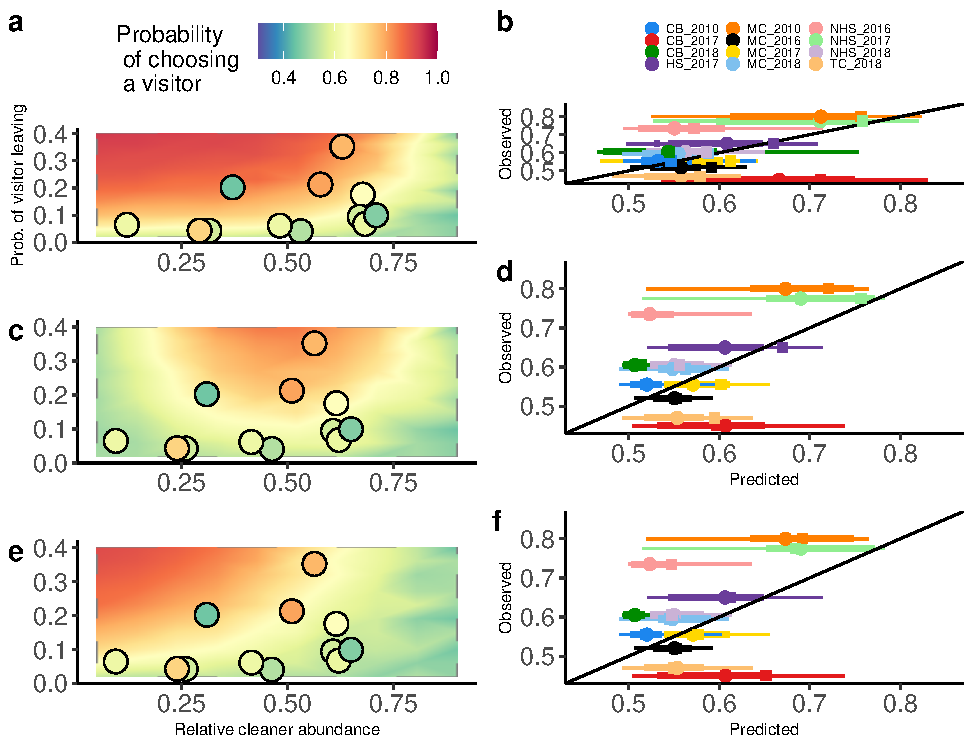
\includegraphics[width=1\linewidth]{manuscript_1.0_files/figure-latex/pred-1} 

}

\caption{Observed and predicted probability of choosing a visitor. Left-hand side panel: color contour shows the prediction of the learning model using the mode of the posterior distributions of parameters recovered by the statistical analysis. Dots show the frequency of visitor choices for the 12 locations, as well as the corresponding relative cleaner abundance (x axis) and frequency of visitors leaving the station (y axis). Right-hand side panels: Variation of the predicted probabilites  of choosing a visitor and their observed values for 12 locations. Circles show the mean prediction for each location from 100 samples taking from the posterior distribution. Thick and thin bars show the 66 and 95\% credible interval taken from those posterior samples. Squares show the predictions used for panel on the righ-hand side. Colour denotes different locations (see Empirical data section). Black line correspond to a perfect match between observed and predicted probabilities. Upper panels show prediction from a model including future and negative reward, lower panels from a  model with only future reward.}\label{fig:pred}
\end{figure}

Figure \ref{fig:pred} shows predictions from the two models. On the
left, the colour coded contour shows the prediction of the model for
combinations of cleaner abundance (x axis) and visitor leaving
probability (y axis). Predictions were generated by running the model
using the mode of the posterior distributions as the parameter values,
and varying systematically cleaner abundance and visitor leaving
probability. Colour of the points on top of the contour show the average
frequency with which cleaner fish chose the visitor plate in their last
20 experimental trials. Each point corresponds to a location with a
combination of cleaner abundance and visitor leaving probability. Panels
on the right show how close the observed values for the probability of
choosing the visitor (y axis) are from the predictions of the models (x
axis). The black line represents the perfect fit between observed and
predicted values. Bars show the variation in predicted values using 100
samples from the posterior distribution. Despite having one more
parameter varying, the full model
gives a lower fit to the data than the model without negative reward.
In the supplementary material, we also show predictions from
model with only negative reward, excluding future rewards (\(\gamma=0\),
Fig. \ref{fig:nogamma}), provides a lower fit than either of the ones
presented in the main text.

The main reason for negative and future reward to give different
predictions is the way that cleaner's relative abundance influences the
preference for the visitor clients. Visitor leaving probability has a
similar positive effect on the probability of choosing the visitor
clients on all three models (Fig. \ref{fig:pred}, \ref{fig:nogamma}). In
contrast, cleaner's relative abundance has a different effect in the
model with only future reward, compared to the other two. In the model
with only future reward only intermediate cleaner abundance triggers a
preference for the visitor clients (Fig. \ref{fig:pred} c). In models
with negative reward, both intermediate and low cleaner abundance
trigger a preference for the visitor. (Fig. \ref{fig:pred} a,
\ref{fig:nogamma}).

\hypertarget{discussion}{%
\subsection{Discussion}\label{discussion}}

We asked which if two potential cognitive mechanisms
-- chaining of events, negative reinforcement, or a combination of both --
is the more likely mechanism to explain intra-specific variation in cleaner
performance in the ephemeral reward task as a function of ecological
conditions in the wild. To evaluate the merits of the alternative mechanisms,
we considered performance in the task to depend on decision-rules that
cleaners had developed in their natural environment: individuals that
solved the task did so because they already had a general preference for
visitors, and applied this rule once being familiar with the task.\\
While all three models capture well the positive relation between visitor
leaving behaviour and cleaner performance in
the market task \citep{triki_Biological_2019}, only the chaining mechanism
predicts that cleaner performance in the task should be low if their
local abundance in the wild relative to clients is low. Indeed, such low
performance is predicted regardless of the visitor leaving
probability. In contrast, a model with negative reward predicts the
highest performance in the ephemeral reward task when relative
cleaner abundance is low, particularly
together with high probability of visitor leaving (Fig. \ref{fig:pred}).
Low cleaner abundances mean the market has an excess of demand for
cleaning services. In the model, this translates to a cleaning station
that is frequently full. Thus, when visitors leave, it's likely that the
cleaner will have access to another client in the next step. Therefore,
there will not be much difference in future reward between choosing
a visitor and a resident, and cleaners will not develop a preference for the
visitor in these conditions. On the other hand, the effect of negative reward
would be opposite as in a full station, cleaners will get more often the
heterotypic (resident-visitor) option and will develop a preference for
the visitor faster. Note that when cleaner abundance is high situations
with a resident and a visitor will be so rare that neither mechanism
will be very efficient in generating a preference for visitors. When
such choice arises it is still be best to choose the visitor; however,
the learning machinery will not be able to develop this preference
efficiently. Overall, estimation of future reward is then the cognitive
mechanism that allows cleaners to adaptively respond to the
ecological conditions of the biological market.

Our results support chaining as the more plausible mechanism behind the
inter-specific variation in cleaners' performance, which is also
the mechanism that allows them to respond more adaptively. This could
suggest chaining to be under positive selection. In the standard ephemeral
reward task, however, food amount and quality are equal between the
two plates. An given that models resemble this, choosing visitors over
residents in low cleaner abundances does not diminish the
amount of food/reward in the the models.
On the other hand, a cleaner committed to visitors might find more difficult
to include in the decision making other variables, like parasite load
and/or mucus quality, that do predict the amount of food in the field
\citep{roche_Client_2021}. In nature and in laboratory experiments, cleaners prefer
higher quality mucus and more food in the absence of market effects
(i.e.~in simultaneous 2-choice options,
\citep{triki_Fluctuations_2019, grutter_Cleaner_2004}), and they use size as a
proxy for food availability \citep{wismer_Cuebased_2019, grutter_Does_2005}.
How important this limitation is will determine whether chaining yields a higher
fitness for cleaners.

Individual cleaners that performed in the laboratory test according to what
is best at their site of capture (low performance when living at low densities,
high performance when living at high densities) had larger forebrains
harbouring more cells than individuals whose performance mismatched locally
optimal decision-rules \citep{triki_Brain_2020}. Triki \emph{et al.} refer to the
former as socially competent cleaners. Social competence refers to the
ability to optimise social behaviour depending on the available social
information \citep{taborsky_Social_2012a, bshary_Cooperation_2015, varela_Correlated_2020}. Our analyses yielded no
evidence that the difference in social competence with respect to the local
market conditions and associated brain morphology are due to the mechanism
used to incorporate future consequences. It could have been conceivable that
high performing individuals from low-density sites might use negative
reinforcement instead of chaining, but in that case negative reinforcement
should have explained part of the data. Configurational learning or
chunking \citep{sutherland_Configural_1989, miller_Magical_1956}, the second component
necessary to solve the ephemeral reward task \citep{quinones_Reinforcement_2019}, was
not varied in the models analized here. However, while chunking tendencies
should vary to allow individuals to adapt to local conditions
\citep{prat_Modelling_2022, kolodny_Evolution_2014}, systematic differences
in individual chunking tendencies would not explain how socially
competent decisions vary as a function of relative abundance.
Therefore, it remains currently unclear what cell-demanding
mechanisms may cause variation in social competence that
translates into site-specific variation in performance in the
ephemeral reward task.

The model is inspired by the general processes of associative learning
where short term rewards are translated to decision making; thus, it
ignores alternative channels of information that could be relevant in
market-like situations. For example, the model does not investigate whether
cleaners actually assess the frequency of client visits or a mean frequency
of visitors leaving. The updating learning mechanism for the development
of preferences works on a trial by trial basis. In the model, cleaners
do not need to assess the actual state of the market, \emph{i.e.} their density,
the density of residents and visitors, and client visitation rate as an
indicator of demand. They only need to assess short-term consequences of
own decisions on food intake and chain them. Also, for the sake of
simplicity, the model ignores the process by which cleaners discriminate
residents and visitor clients. A model that accounts for this discrimination
probably involves the development of preferences for morphological or
behavioural features that are statistically associated with visitors
or residents. For example, visitors are on average larger larger
than residents \citep{bshary_Cleaner_2001a}, and are less likely to chase
cleaners in response to the latter cheating by taking a bite of
mucus \citep{bshary_Asymmetric_2002}. Given these associations, chaining might
produce the decision-rule ``chose the larger client and/or less aggressive
client'', which does not help in the standard ephemeral reward task.

In conclusion, our study shows that variation in cognitive performance as
a function of ecological factors may set the stage for the use of
mechanistic modelling to identify the cognitive processes underlying
learning in animals. The combination overcomes the limitations
of the general philosophy in animal cognition to apply the logic of
Lloyd Morgen's canon (Occam's razor). Excluding basic
reinforcement learning explanations (operant and/or classical conditioning)
as a potential explanation in experiments
often warrants animals solving the task on the first possible occasion.
For example, any theory of mind task needs to be solved in the first
trial in order to exclude fast conditioning \citep{heyes_Theory_1998}.
Similarly, subjects need to solve a social learning task on the first
trial to accept imitation as a mechanism over stimulus/local
enhancement. Such strict conditions are virtually never met. For
example, potato washing by Japanese macaques, an iconic example of
social learning, took several years to spread within the group
\citep{kawamura_Process_1959}, meaning that any learner had been repeatedly
exposed to demonstrations before acquisition. Importantly, Galef
\citep{galef_Question_1992} refuted imitation as mechanism not simply because
of the repeated exposure but because a (rather qualitative) analysis of
the spread of potato washing across individuals did not follow the
prediction based on imitation learning (see also
\citep{hirata_SweetPotato_2001}). In our case, the number of trials it took
cleaners to learn the solution to the market task would never allow to
exclude an important role of negative reinforcement based on the data
alone. However, fitting model predictions to our data set revealed that
a more complex mechanism (estimation of future reward) fits the data
better.

\newpage

\hypertarget{supplementary-material}{%
\section{Supplementary material}\label{supplementary-material}}

\beginsupplement

\begin{figure}[H]

{\centering 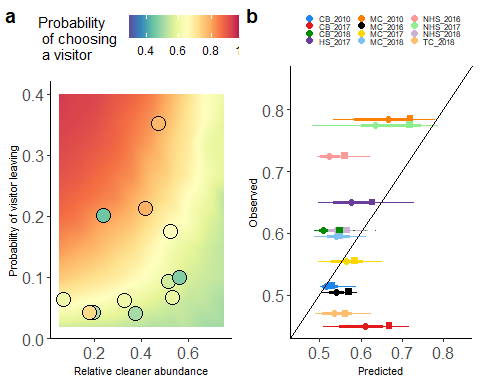
\includegraphics[width=0.95\linewidth,]{manuscript_1.0_files/figure-latex/nogamma-1} 

}

\caption{Observed and predicted probability of choosing a visitor for a model without future rewards. Left-hand side panel: color contour shows the prediction of the learning model using the mode of the posterior distributions of parameters recovered by the statistical analysis. Dots show the frequency of visitor choices for the 12 locations, as well as the corresponding relative cleaner abundance (x axis) and frequency of visitors leaving the station (y axis). Right-hand side panel: Right-hand side panels: Variation of the predicted probabilites  of choosing a visitor and their observed values for 12 locations. Circles show the mean prediction for each location from 100 samples taking from the posterior distribution. Thick and thin bars show the 66 and 95\% credible interval taken from those posterior samples. Squares show the predictions used for panel on the righ-hand side. Colour denotes different locations (see Empirical data section). Black line correspond to a perfect match between observed and predicted probabilities.}\label{fig:nogamma}
\end{figure}

\begin{longtable}[]{@{}rc@{}}
\caption{\label{tab:param} Parameter values with which the model was run
in the MCMC. \(\sigma\) refers to the amplitud of the perturbation kernel with the subscript indicating the associated parameter. New values were taken from a uniform distribution. \(\alpha\) refers to the learning rate.}\tabularnewline
\toprule
Parameter & Value \\
\midrule
\endfirsthead
\toprule
Parameter & Value \\
\midrule
\endhead
Learning rounds & 10000 \\
Reward value & 1 \\
\(\alpha\) & 0.05 \\
\(\sigma_{\gamma}\) & 0.3 \\
\(\sigma_{\eta}\) & 4 \\
\(\sigma_{Sca.Const.}\) & 300 \\
Number of chains & 5 \\
Chain lenght & \(1^5\) \\
\bottomrule
\end{longtable}

\ethics{The Animal Ethics Committee of the Queensland government (DAFF)
approved the project (CA 2016/05/970 and CA 2017/05/1063).}

\dataccess{Please provide details on the data availability.}

\aucontribute{AQ and RB designed the study. ZT collected the data. AQ developed the model and
fitted the model parameters to the data. AQ, RB and ZT wrote the manuscript.}

\competing{The authors declate no conflict of interests.}

\funding{This work was supported by the Swiss National Science Foundation (grants
number: 31003A\_153067/1 and 310030B\_173334/1 to R.B.).}


\ack{ZT and RB kindly thank the staff of Lizard Island Research Station, Dominique
Roche, Sharon Wismer, Olivia Rey,Sandra Ann Binning, Elena Levorato and William McNeely for their
field support. AQ thanks Florian Hartig for statistical advice.}

\bibliographystyle{RS}
\bibliography{Cleanerlearning.bib}


\end{document}
